\documentclass{amsart}
\usepackage{graphicx}
\usepackage{geometry}[margins=.5in]

\begin{document}
\section{Problem 1}
For the dataset given on Blackboard, the following summary statistics were calculated.

\begin{table}[ht]
\centering
\begin{tabular}{ll}
  \hline
Statistic & Value \\
  \hline
Mean & $1688.51$ \\
Median & $1706$ \\
Std. Dev & $883.47$ \\
Max & $3907$ \\
Min & $2$ \\
   \hline
\end{tabular}
\end{table}

The histogram for the dataset can be found in Figure~\ref{fig:p1a}

\begin{figure}
  \centering
  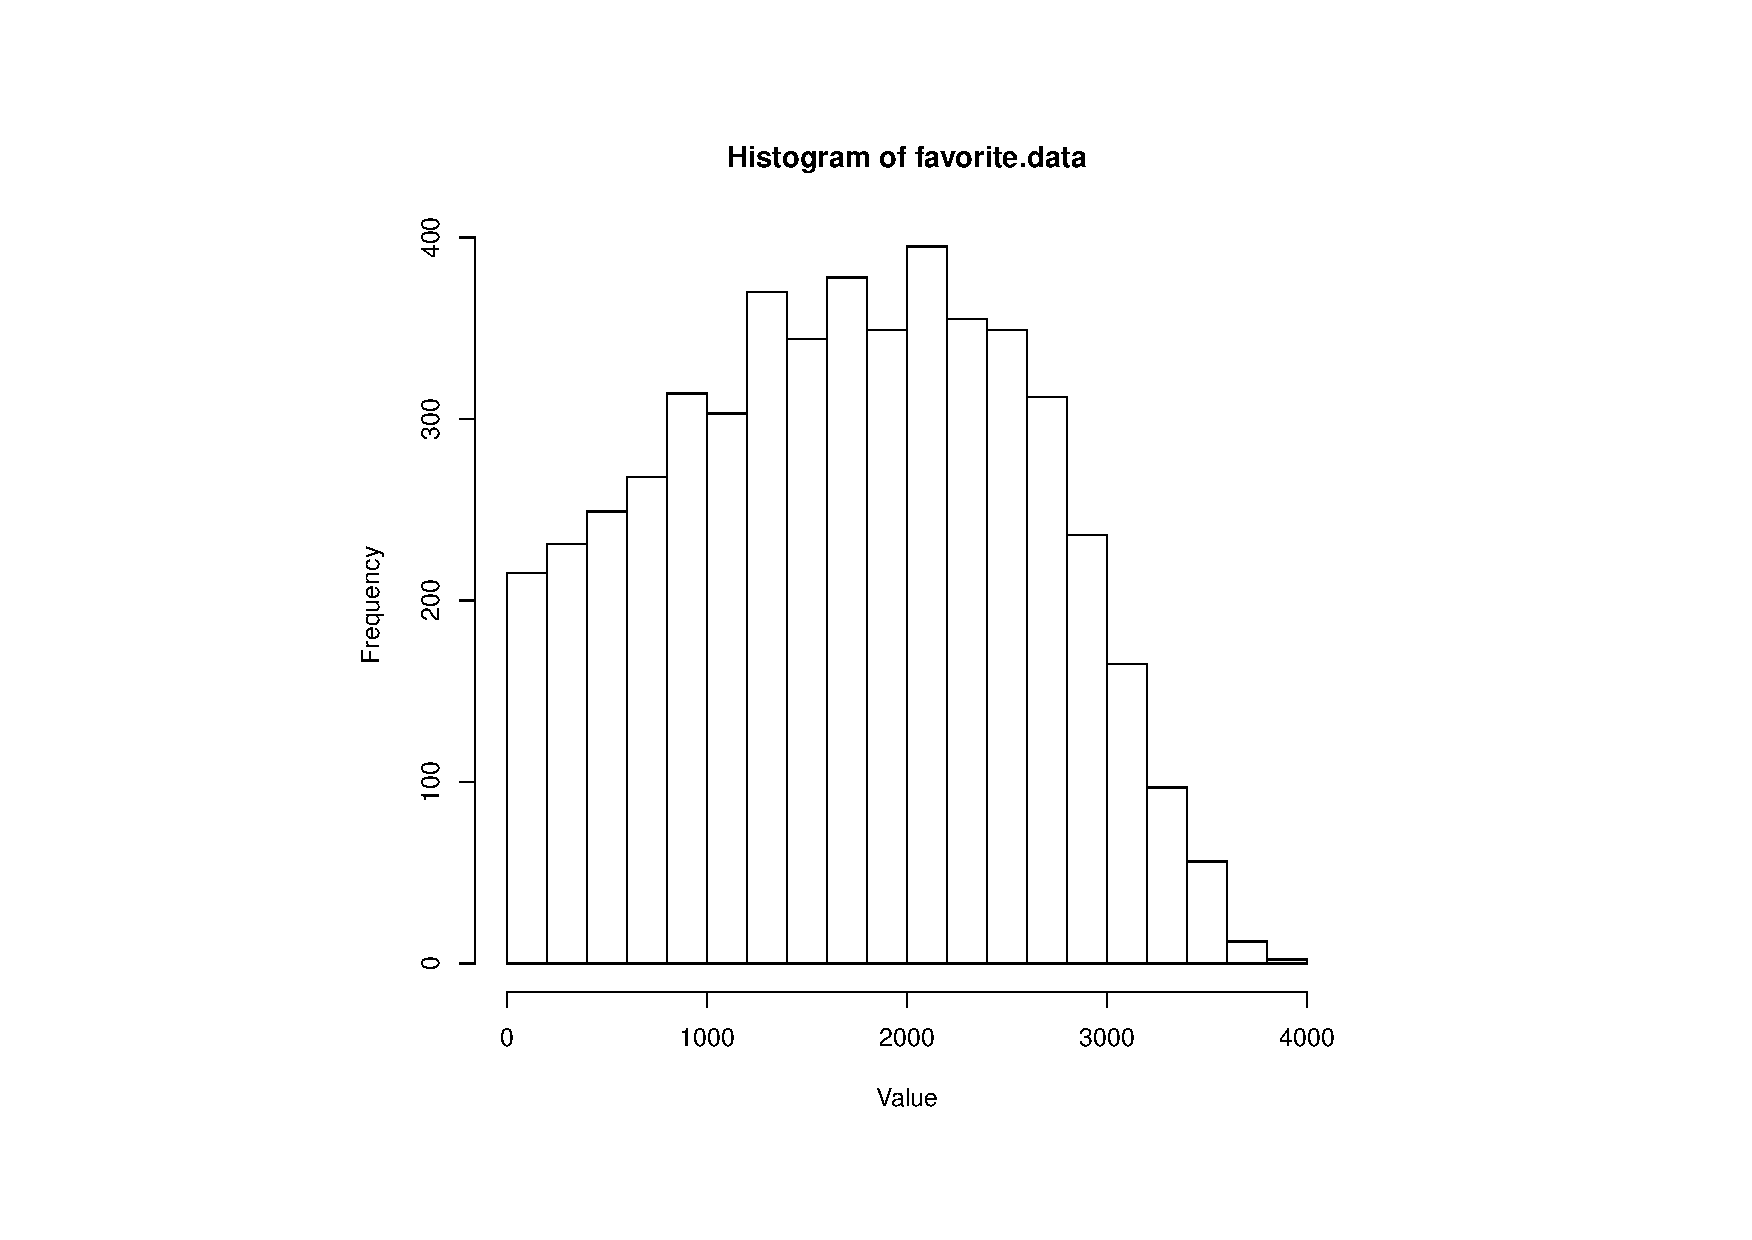
\includegraphics[width=\linewidth]{problem1_histogram.pdf}
  \caption{The histogram of favorite.data}
  \label{fig:p1a}
\end{figure}


\section{Problem 2}
We generate 10,000 random values from the standard normal
distribution. The histogram of the values is shown below in Figure~\ref{fig:p2a}.
\begin{figure}
  \centering
  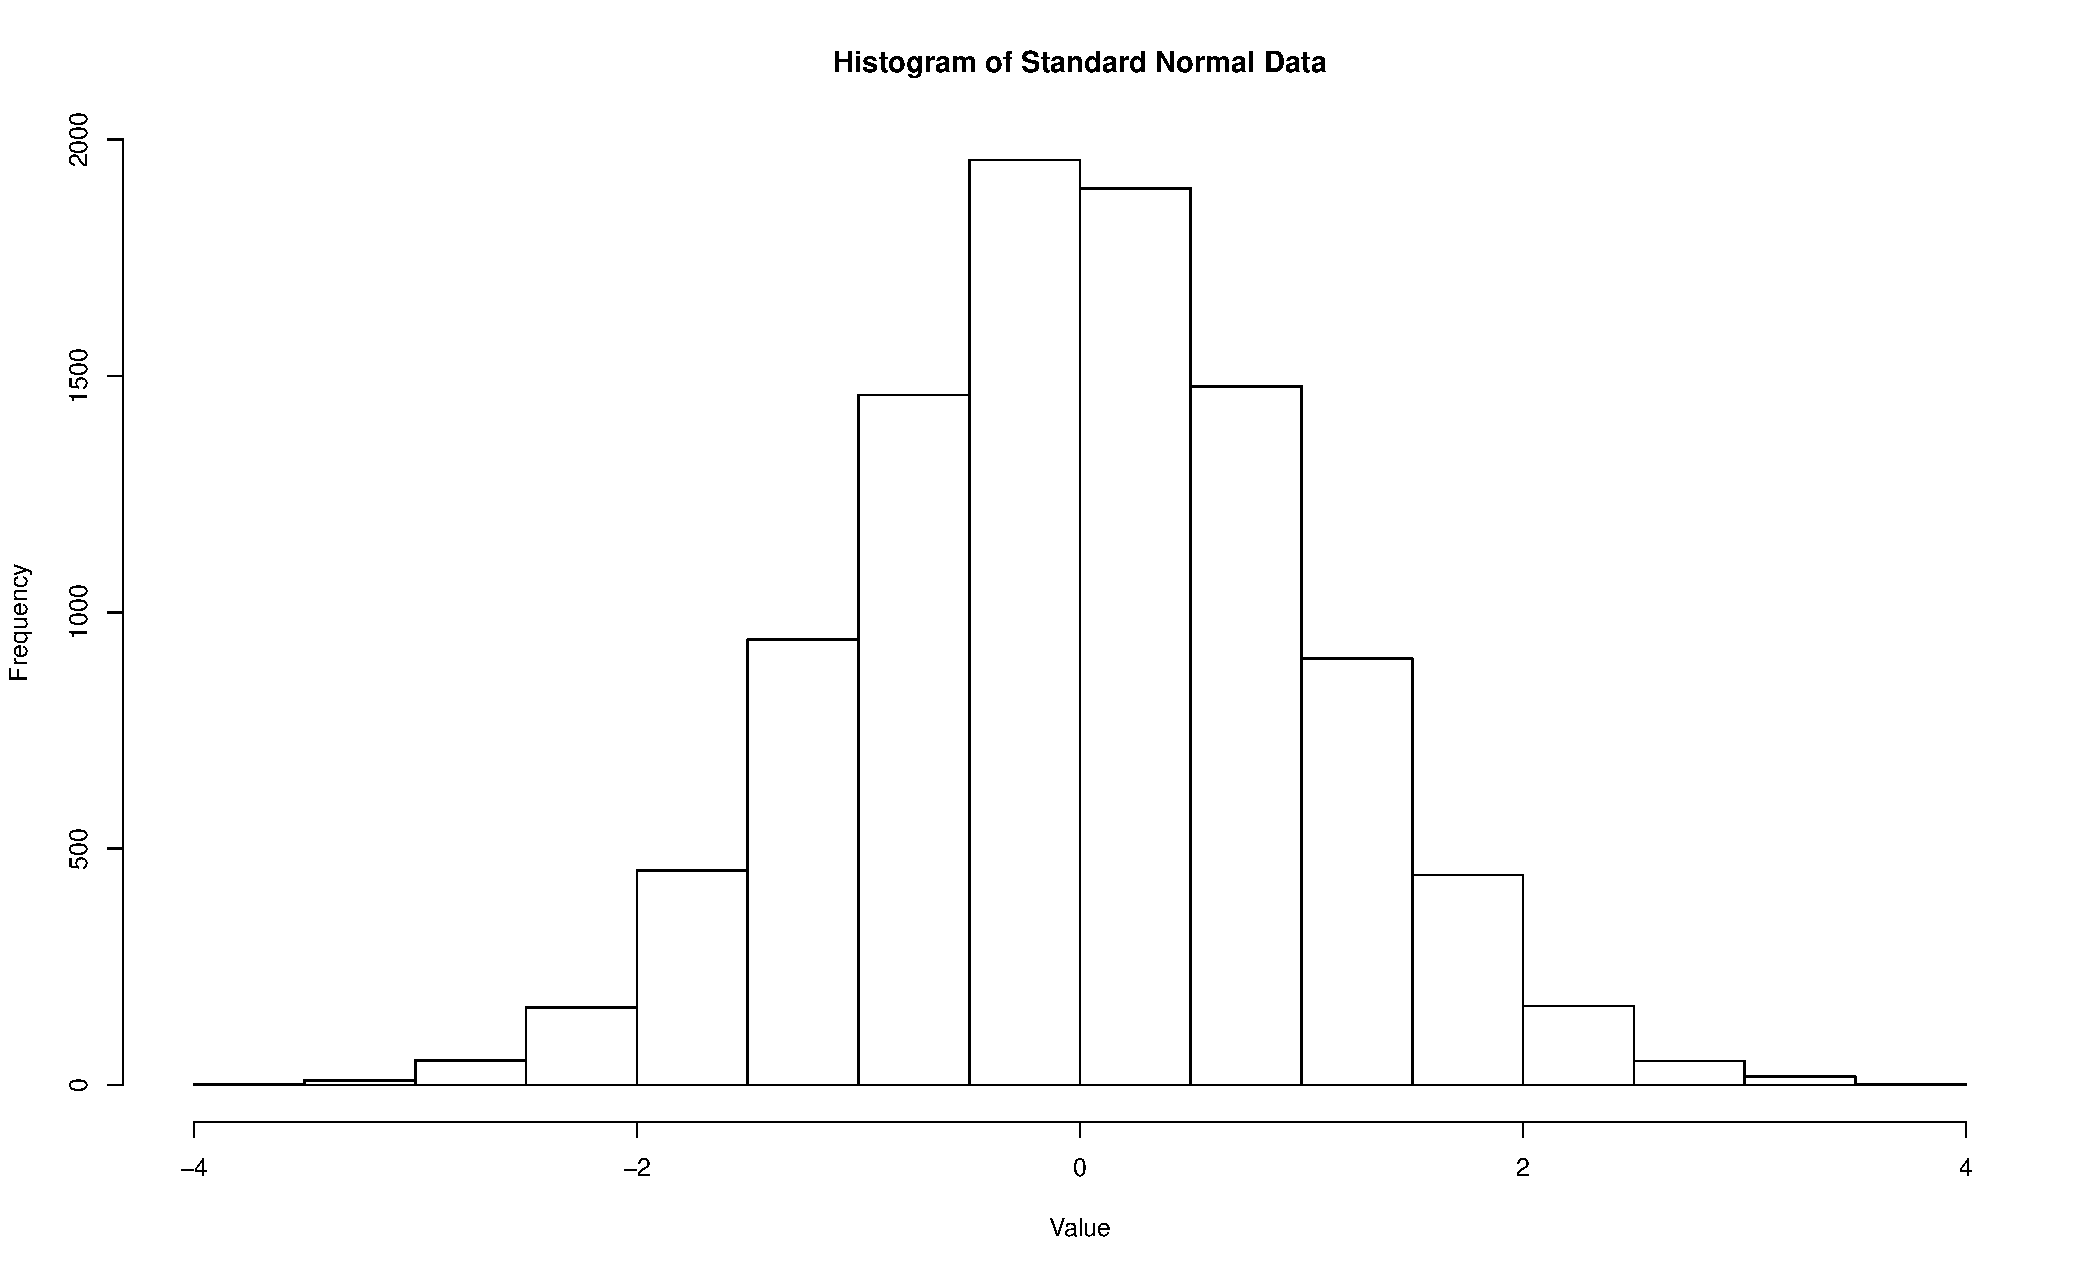
\includegraphics[width=\linewidth]{problem2_histogram.pdf}
  \caption{The histogram of 10,000 random standard normal data points}
  \label{fig:p2a}
\end{figure}

The following statistics were calculated.
\begin{table}[ht]
\centering
\begin{tabular}{ll}
  \hline
Statistic & Value \\
  \hline
Mean & $-0.0032$ \\
Median & $-.00966$ \\
Std. Dev & $1.00658$ \\
   \hline
\end{tabular}
\end{table}

\section{Problem 3}
The two sequences specified in the problem were multiplied together.
The requested elements can be found in the table below.

\begin{table}[ht]
\centering
\begin{tabular}{ll}
  \hline
Element & Value \\
  \hline
15 & $5475$ \\
16 & $5760$ \\
17 & $6035$ \\
   \hline
\end{tabular}
\end{table}

All of the elements between 5 and 32 (inclusive) are greater than 2,000.

16 elements are greater than 6,000.

\section{Problem 4}
The following table describes the results of summing all of the perfect
squares between 1 and $x$.
\begin{table}[ht]
\centering
\begin{tabular}{ll}
  \hline
    $x$ & Value \\
  \hline
  $100$ & $385$ \\
  $100,000$ & $10568146$ \\
   \hline
\end{tabular}
\end{table}

\section{Problem 5}
All of the perfect squares between 1 and 500 can be found in the table below
(code with the vector object in the appendix).
\begin{table}[ht]
\centering
\begin{tabular}{ll}
  \hline
 & x \\
  \hline
1 & 1.00 \\
  2 & 4.00 \\
  3 & 9.00 \\
  4 & 16.00 \\
  5 & 25.00 \\
  6 & 36.00 \\
  7 & 49.00 \\
  8 & 64.00 \\
  9 & 81.00 \\
  10 & 100.00 \\
  11 & 121.00 \\
  12 & 144.00 \\
  13 & 169.00 \\
  14 & 196.00 \\
  15 & 225.00 \\
  16 & 256.00 \\
  17 & 289.00 \\
  18 & 324.00 \\
  19 & 361.00 \\
  20 & 400.00 \\
  21 & 441.00 \\
  22 & 484.00 \\
   \hline
\end{tabular}
\end{table}

The 4 column matrix with all perfect squares between 1 and 100,000
can be found below (code in the appendix).
\begin{table}[ht]
\centering
\begin{tabular}{lllll}
  \hline
 & 1 & 2 & 3 & 4 \\
  \hline
1 & 1.00 & 6400.00 & 25281.00 & 56644.00 \\
  2 & 4.00 & 6561.00 & 25600.00 & 57121.00 \\
  3 & 9.00 & 6724.00 & 25921.00 & 57600.00 \\
  4 & 16.00 & 6889.00 & 26244.00 & 58081.00 \\
  5 & 25.00 & 7056.00 & 26569.00 & 58564.00 \\
  6 & 36.00 & 7225.00 & 26896.00 & 59049.00 \\
  7 & 49.00 & 7396.00 & 27225.00 & 59536.00 \\
  8 & 64.00 & 7569.00 & 27556.00 & 60025.00 \\
  9 & 81.00 & 7744.00 & 27889.00 & 60516.00 \\
  10 & 100.00 & 7921.00 & 28224.00 & 61009.00 \\
  11 & 121.00 & 8100.00 & 28561.00 & 61504.00 \\
  12 & 144.00 & 8281.00 & 28900.00 & 62001.00 \\
  13 & 169.00 & 8464.00 & 29241.00 & 62500.00 \\
  14 & 196.00 & 8649.00 & 29584.00 & 63001.00 \\
  15 & 225.00 & 8836.00 & 29929.00 & 63504.00 \\
  16 & 256.00 & 9025.00 & 30276.00 & 64009.00 \\
  17 & 289.00 & 9216.00 & 30625.00 & 64516.00 \\
  18 & 324.00 & 9409.00 & 30976.00 & 65025.00 \\
  19 & 361.00 & 9604.00 & 31329.00 & 65536.00 \\
  20 & 400.00 & 9801.00 & 31684.00 & 66049.00 \\
  21 & 441.00 & 10000.00 & 32041.00 & 66564.00 \\
  22 & 484.00 & 10201.00 & 32400.00 & 67081.00 \\
  23 & 529.00 & 10404.00 & 32761.00 & 67600.00 \\
  24 & 576.00 & 10609.00 & 33124.00 & 68121.00 \\
  25 & 625.00 & 10816.00 & 33489.00 & 68644.00 \\
  26 & 676.00 & 11025.00 & 33856.00 & 69169.00 \\
  27 & 729.00 & 11236.00 & 34225.00 & 69696.00 \\
  28 & 784.00 & 11449.00 & 34596.00 & 70225.00 \\
  29 & 841.00 & 11664.00 & 34969.00 & 70756.00 \\
  30 & 900.00 & 11881.00 & 35344.00 & 71289.00 \\
  31 & 961.00 & 12100.00 & 35721.00 & 71824.00 \\
  32 & 1024.00 & 12321.00 & 36100.00 & 72361.00 \\
  33 & 1089.00 & 12544.00 & 36481.00 & 72900.00 \\
  34 & 1156.00 & 12769.00 & 36864.00 & 73441.00 \\
  35 & 1225.00 & 12996.00 & 37249.00 & 73984.00 \\
  36 & 1296.00 & 13225.00 & 37636.00 & 74529.00 \\
  37 & 1369.00 & 13456.00 & 38025.00 & 75076.00 \\
  38 & 1444.00 & 13689.00 & 38416.00 & 75625.00 \\
  39 & 1521.00 & 13924.00 & 38809.00 & 76176.00 \\
  40 & 1600.00 & 14161.00 & 39204.00 & 76729.00 \\
  41 & 1681.00 & 14400.00 & 39601.00 & 77284.00 \\
  42 & 1764.00 & 14641.00 & 40000.00 & 77841.00 \\
  43 & 1849.00 & 14884.00 & 40401.00 & 78400.00 \\
  44 & 1936.00 & 15129.00 & 40804.00 & 78961.00 \\
  45 & 2025.00 & 15376.00 & 41209.00 & 79524.00 \\
  46 & 2116.00 & 15625.00 & 41616.00 & 80089.00 \\
  47 & 2209.00 & 15876.00 & 42025.00 & 80656.00 \\
  48 & 2304.00 & 16129.00 & 42436.00 & 81225.00 \\
  49 & 2401.00 & 16384.00 & 42849.00 & 81796.00 \\
  50 & 2500.00 & 16641.00 & 43264.00 & 82369.00 \\
  51 & 2601.00 & 16900.00 & 43681.00 & 82944.00 \\
  52 & 2704.00 & 17161.00 & 44100.00 & 83521.00 \\
  53 & 2809.00 & 17424.00 & 44521.00 & 84100.00 \\
  54 & 2916.00 & 17689.00 & 44944.00 & 84681.00 \\
  55 & 3025.00 & 17956.00 & 45369.00 & 85264.00 \\
  56 & 3136.00 & 18225.00 & 45796.00 & 85849.00 \\
  57 & 3249.00 & 18496.00 & 46225.00 & 86436.00 \\
  58 & 3364.00 & 18769.00 & 46656.00 & 87025.00 \\
  59 & 3481.00 & 19044.00 & 47089.00 & 87616.00 \\
  60 & 3600.00 & 19321.00 & 47524.00 & 88209.00 \\
  61 & 3721.00 & 19600.00 & 47961.00 & 88804.00 \\
  62 & 3844.00 & 19881.00 & 48400.00 & 89401.00 \\
  63 & 3969.00 & 20164.00 & 48841.00 & 90000.00 \\
  64 & 4096.00 & 20449.00 & 49284.00 & 90601.00 \\
  65 & 4225.00 & 20736.00 & 49729.00 & 91204.00 \\
  66 & 4356.00 & 21025.00 & 50176.00 & 91809.00 \\
  67 & 4489.00 & 21316.00 & 50625.00 & 92416.00 \\
  68 & 4624.00 & 21609.00 & 51076.00 & 93025.00 \\
  69 & 4761.00 & 21904.00 & 51529.00 & 93636.00 \\
  70 & 4900.00 & 22201.00 & 51984.00 & 94249.00 \\
  71 & 5041.00 & 22500.00 & 52441.00 & 94864.00 \\
  72 & 5184.00 & 22801.00 & 52900.00 & 95481.00 \\
  73 & 5329.00 & 23104.00 & 53361.00 & 96100.00 \\
  74 & 5476.00 & 23409.00 & 53824.00 & 96721.00 \\
  75 & 5625.00 & 23716.00 & 54289.00 & 97344.00 \\
  76 & 5776.00 & 24025.00 & 54756.00 & 97969.00 \\
  77 & 5929.00 & 24336.00 & 55225.00 & 98596.00 \\
  78 & 6084.00 & 24649.00 & 55696.00 & 99225.00 \\
  79 & 6241.00 & 24964.00 & 56169.00 & 99856.00 \\
   \hline
\end{tabular}
\end{table}

For the above matrix $\bf{X}$, $x_{15, 3}$ = 29,929.



\end{document}
